% Chapter 1

\chapter{Cryptography} % Main chapter title

\label{EC} % For referencing the chapter elsewhere, use \ref{Chapter1} 

%----------------------------------------------------------------------------------------

% Define some commands to keep the formatting separated from the content 
\newcommand{\keyword}[1]{\textbf{#1}}
\newcommand{\tabhead}[1]{\textbf{#1}}
\newcommand{\code}[1]{\texttt{#1}}
\newcommand{\file}[1]{\texttt{\bfseries#1}}
\newcommand{\option}[1]{\texttt{\itshape#1}}

%----------------------------------------------------------------------------------------

In order to have a clear understanding of this thesis, it is necessary to know the basic concepts of:
\begin{itemize}[label=$\checkmark$]
	\item HASH function.
	\item Elliptic Curve.
\end{itemize}
Only these two elements together can describe all the cryptography behind Bitcoin.

\section{HASH function}
In general, a hash function is a mathematical process that takes input data of \textit{any} size, performs an operation on it, and returns output data of a \textit{fixed} size.
\\ \\
The input data is called \textit{message} and the output data is called \textit{hash value}. 
\\ \\
A good and secure hash function must have at least these six properties:
\begin{enumerate}[label=(\roman*)]
	\item It is \textbf{deterministic}: if the message remains unchanged, the hash value is the same.
	\item It is \textbf{quick}: it should not take too much time to compute the hash value from the message.
	\item It is a \textbf{ONE-WAY function}: it is infeasible to find a message, knowing the hash value. The only way to find the message must be to try randomly all the possible combination.
	\item It is \textbf{collision free}: it is infeasible to find two messages with the same hash value, even if it is theoretically possible.
	\item It has the \textbf{avalanche effect}: a very small change in the input message, even flipping a single bit, produces a completely different hash value.
	\item It has \textbf{fixed size} output and could have input messages of \textbf{any size}.
\end{enumerate}
In this thesis, we will see hash functions as black-boxes, with all the proprieties described above. 
\\ \\
There are various kinds, but for our purpose, the main difference lies in the number of bits of the hash value. Among all the possible hash functions, in Bitcoin cryptography three functions are used:
\begin{itemize}
	\item \textbf{SHA256}: Secure Hash Algorithm 256
	\begin{itemize}
		\item developed by the National Institute of Standards and Technology (NIST) as a U.S. Federal Information Processing Standard (FIPS).
		\item output size: 256 bits.
	\end{itemize}
	\item \textbf{SHA512}: Secure Hash Algorithm 512
	\begin{itemize}
		\item developed by the National Institute of Standards and Technology (NIST) as a U.S. Federal Information Processing Standard (FIPS).
		\item output size: 512 bits.
	\end{itemize}
	\item \textbf{RIPEDM160}: RACE Integrity Primitives Evaluation Message Digest 160
	\begin{itemize}
		\item developed by Hans Dobbertin, Antoon Bosselaers and Bart Preneel at the COSIC research group at the Katholieke Universiteit Leuven. 
		\item output size: 160 bits.
	\end{itemize}
\end{itemize}
One important hash function used in the Bitcoin cryptography is the so-called HASH160. It is simply the concatenation of SHA256 and RIPEDM160:
\begin{equation*}
HASH160 \, (\, msg\, ) = RIPEDM160\, (\, SHA256 \, (\, msg \, )).
\end{equation*}
From the moment that the last operation made to compute the HASH160 function was the RIPEDM160 function, the output size is 160 bits.

\subsection{Other functions}

There are two other functions that will be heavily used in this thesis:
\begin{itemize}
	\item \textbf{HMAC}: Hash-based Message Authentication Code,
	\item \textbf{PBKDF2}: Password-Based Key Derivation Function 2.
\end{itemize}
\begin{flushleft}
	\textbf{HMAC} is a function that made some computation, involving also a hash function. This algorithm provides better immunity against \textit{length extension attacks}, namely attack in which the length of the input message is known and all the possible combinations of the input are tried.
\end{flushleft}
It receives 3 inputs:
\begin{itemize}[label=$\odot$]
	\item \textbf{Hash function}: a hash function with the properties described above.
	\item \textbf{Key}: a sequence of bytes.
	\item \textbf{Message}: a sequence of bytes.
\end{itemize}
This function computes the following operations:
\begin{equation*}
HMAC(H,k,m)=H\, (\, opad(k) \, ||\, H\, (\, ipad(k) \, ||\,  m \, )),
\end{equation*}
where $H$ is the hash function, $k$ is the key, $m$ is the message, $opad(\bullet)$ and $ipad(\bullet)$ are two padding function, applied to the key $k$ and $||$ is a symbol that denotes concatenation.
\\ \\
\textbf{PBKDF2} is an algorithm that applied a hash function to an input (message) many times. Each of these times a particular string of bytes, called \textit{salt}, is inserted within the computation of the hash. This algorithm provides more computational work with respect to a single hash function, and so it reduces the risk of a brute force attack.
\\ \\
It receives five inputs:
\begin{itemize}[label=$\odot$]
	\item \textbf{Message}: a sequence of bytes.
	\item \textbf{Salt}: a sequence of bytes.
	\item \textbf{Number of iterations}: the number of iteration to be computed.
	\item \textbf{Digest-module}: a hash function with the properties described above.
	\item \textbf{Mac-module}: a message authentication code  module (e.g. HMAC).
\end{itemize}
Having a salt reduces the ability to use rainbow tables for attacks, namely tables with precomputed hash value. It is recommended to use at least 64 bits for the salt.







\section{Elliptic Curve over $\mathbb{F}_p$}
Elliptic curve [\cite{7,8,9,10}] is a \textit{plane algebraic curve} defined by an equation, over a specific field. In cryptography the field is finite.
\\ \\
A point $Q$, which coordinates are $x$ and $y\in \mathbb{N}$, belong to an Elliptic Curve if and only if $Q$ satisfies the following equation:
\begin{equation}\label{GeneralEC}
y^2=x^3+ax+b \quad \textrm{over} \ \mathbb{F}_p,
\end{equation}
where $\mathbb{F}_p$ is the finite field defined over the set of integers modulo $p$ and $a$ and $b$ are the coefficients of the curve. \\ \\
We can rewrite the Equation (\ref{GeneralEC}) in the following way:

\begin{equation}\label{GeneralECmodp}
y^2=x^3+ax+b \quad \textrm{mod} \ p.
\end{equation}
Figure \ref{fig:EC_ex} shows some examples of Elliptic Curve over $\mathbb{F}_p$ with $a=-7$ and $b=10$
\begin{figure}[ht!]
	\centering
	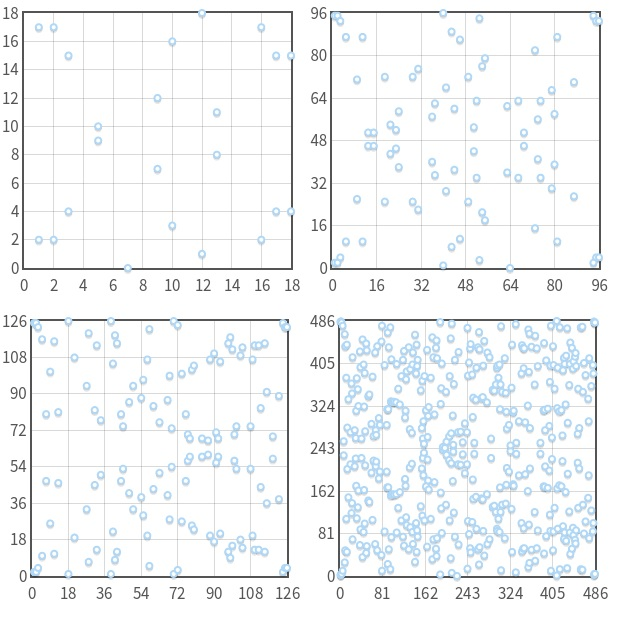
\includegraphics[width=9cm]{Figures/EC_ex.jpg}
	\caption{Points on the Elliptic Curve $y^2=x^3-7x+10 \; \textrm{mod} \ p$, with $p=19,97,127,487$ }
	\label{fig:EC_ex}
\end{figure}

\subsection{Symmetry}
The elliptic curve has an important property: the line $y=p/2$ is an axis of symmetry for the curve.
\\ \\
This can be shown, by proving that the point $P(x,y)$ belongs to the Elliptic Curve ($EC$) if and only if the point $Q(x,p-y)$ belongs to the curve too:
\begin{equation*}
P(x,y) \in EC \iff Q(x,p-y) \in EC.
\end{equation*}
\textit{Proof}:
\\ \\
First analyze the implication in the right direction: ($\implies $).
\\ \\
From Equation (\ref{GeneralECmodp}) and from the hypothesis we have that:
\begin{equation*}
P(x,y) \in EC \implies y^2=x^3+ax+b \quad \textrm{mod} \ p,
\end{equation*}
but we know also that: 
\begin{equation*}
Q(x,p-y) \in EC \iff (p-y)^2=x^3+ax+b \quad \textrm{mod} \ p.
\end{equation*}
From the moment that the right hand side of both the equations are equal, we only need to prove that:
\begin{equation*}
(p-y)^2=y^2 \quad \textrm{mod} \ p.
\end{equation*}
This is true, indeed:
\begin{align*}
(p-y)^2 & = p^2 -2py + y^2 &  \textrm{mod} \ p \\
& = p\cdot(p -2y) + y^2 &  \textrm{mod} \ p \\
& = 0+y^2 &  \textrm{mod} \ p \\
& = y^2 &  \textrm{mod} \ p
\end{align*}
This is due to the fact that 
\begin{equation*}
p\cdot k =0 \quad \textrm{mod} \ p \qquad \forall k\in \mathbb{N}.
\end{equation*}
The other implication ($\impliedby$) is almost the same and it follows the same logic.
\begin{flushright}
	\textit{c.v.d.}
\end{flushright}
Once shown the symmetry property, it can be useful to denote the point $P(x,y)$ as the opposite of $Q(x,p-y)$:
\begin{equation*}
P=-Q \implies P+Q=0,
\end{equation*}
where the $+$ operator between two points in the EC will be explained below and the $0$ in this contest is the \textit{point at infinity}.

\subsection{Point addition}
Once defined a point on the elliptic curve, let's introduce the addition between two points on this finite field.
\\ \\
We need to change our definition of addition in order to make it works in $\mathbb{F}_p$. In this framework, we claim that if some points are aligned over the finite field $\mathbb{F}_p$, then they have zero-sum.
\\ \\
So $P+Q=R$ if and only if $P$, $Q$ and $-R$ are aligned, in the sense shown in Figure \ref{fig:EC_aligned}
\begin{figure}[ht!]
	\centering
	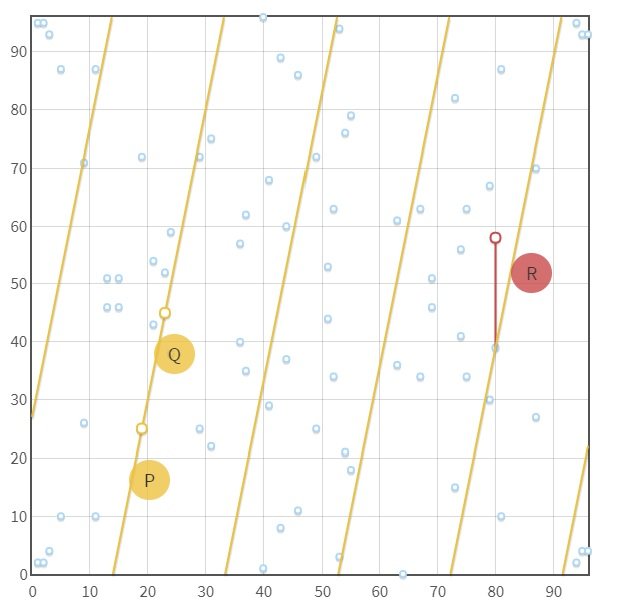
\includegraphics[width=9cm]{Figures/EC_aligned.jpg}
	\caption{Elliptic Curve $y^2=x^3-7x+10 \; \textrm{mod} \ 97$}
	\label{fig:EC_aligned}
\end{figure}

\begin{flushleft}
	After defined when points in the EC have zero-sum, it is possible to calculate the equations for point addition:
\end{flushleft}
Suppose that \textit{A} and \textit{B} belong to the Elliptic Curve.

\begin{center}
	$ A=(x_1,y_1) \quad B=(x_2,y_2)$.
\end{center}
Let's define $ A+B :=(x_3,y_3) $ 
\\ \\
When $x_1=x_2$ but $y_1 \neq y_2$, it is the case in which $A$ and $B$ are symmetric point and so the sum is a particular point, called \textit{point at infinity}: 
\begin{equation*}
A+B=0=	(inf,inf) .
\end{equation*}
In all the other cases we have:



\begin{center} 
	$s=\begin{cases} \dfrac{y_2-y_1}{x_2-x_1}, & \mbox{if } x_1\neq x_2, \; y_1\neq y_2 \;\rightarrow \; \text{point addition},\\ \\ \dfrac{3x_1^2+a}{2y_1}, & \mbox{if } x_1= x_2, \; y_1= y_2 \;\rightarrow \; \text{point doubling}, \end{cases}$
\end{center}
where $s$ is a dummy variable, used to compute $x_3$ and $y_3$. It can be computed in two different way: if we are performing a "real" point addition, when $A\neq B$ or if we are looking for the double of a point, when $A= B$.
\begin{center} 
	$ x_3=s^2-x_1-x_2  \quad$ mod $p$,\\
	$y_3=s(x_1-x_3)-y_1  \quad$mod $p$.
\end{center}
Once we have $s$ the value $x_3$ and $y_3$ are obtained following this simple formula.


\subsection{Scalar multiplication}
Once defined the addition, any multiplication between a scalar and a point on the elliptic curve can be defined as:
\begin{center} 
	$ nP=\underbrace{
		P+P+\cdot \cdot \cdot+P
	}_{n\text{ times}}$.
\end{center}
When $n$ is a very large number can be difficult or even infeasible to compute $nP$ in this way, but we can use the \textit{double and add algorithm} in order to perform multiplication in $\mathcal{O}(\log{}n)$ steps. Let's see an example:
\\ \\
Suppose that we need to compute $53 \cdot P$ where $P$ is a point on the EC:
\begin{equation*}
53 \cdot P = 110101_{base\, 2} \cdot P = 2^{5}\cdot P + 2^{4}\cdot P + 2^{2}\cdot P + P
\end{equation*}
Computing the common sub-terms only once we obtain a total of 5 doubling and 3 addition operations, much less of 52 addition operations. This algorithm is even more efficient if the scalar is a very large number.

\subsection{Discrete Logarithm Problem}
Once we have described the multiplication between a scalar and a point, let's see if it is possible to make the inverse operation. Let's suppose that:
\begin{equation*}
Q = n \cdot P,
\end{equation*}
where $Q$ and $P$ are points on the EC and $n$ is a scalar number. 
\\ \\ 
Let's suppose to know $Q$ and $P$. With these information it exists only one possible $n \in \mathbb{N}$, such that $0<n<p$ and that the equation above holds true. Even so this number $n$ is infeasible to find for large value of $p$.
\\ \\
This is due to the fact that there is not an efficient algorithm that is able to compute $n$ given $P$ and $Q$. The only way to find $n$ is by trying. As already mentioned, this could become infeasible if the number of value that $n$ can assume ($p-1$) is too large.

\subsection{Group order}
An elliptic curve defined over a finite field is a group and so it has a finite number of points. This number is called \textit{order} of the group.
\\ \\
If $p$ is a very large number, it is impossible to count all the points in that field, but there is an algorithm that allows to calculate the \textit{order} of a group in a fast and efficient way: \textit{Schoof's algorithm}.
\\ \\
Let's consider a generic point $G$, we have:
\begin{center} 
	$ nG+mG=\underbrace{
		G+\cdot \cdot \cdot+G
	}_{n\text{ times}}+
	\underbrace{
		G+\cdot \cdot \cdot+G
	}_{m\text{ times}}=
	\underbrace{
		G+\cdot \cdot \cdot+G
	}_{n+m\text{ times}} = 
	(n+m)G$.
\end{center}
So multiples of $G$ are closed under addition and this is enough to prove that the set of the multiples of $G$ is a cyclic subgroup of the group formed by the elliptic curve.
\\ \\
The point $G$ is called \textbf{generator} of the cyclic subgroup.

\begin{remark}
	The order of the subgroup generated by $G$ is linked to the order of the elliptic curve by Lagrange's theorem, which states that the order of a subgroup is a divisor of the order of the parent group.
\end{remark}

\begin{remark}
	If the order of the group is a prime number, all the points belonging to the EC generate a subgroup with the same order of the group or with order 1.
\end{remark}
All these preliminary information are needed in order to introduce the private-public key cryptography used by Bitcoin.





\subsection{Bitcoin private-public key cryptography}

Bitcoin [\cite{11}] uses a specific Elliptic Curve defined over the finite field of the natural numbers, where $a=0$ and $b=7$.\\ \\
The Equation (\ref{GeneralEC}) becomes:
\begin{equation}\label{BitcoinEC}
y^2=x^3+7 \quad \textrm{mod} \ p,
\end{equation}
where the \textit{mod p} (modulo prime number) indicates that this curve is over a finite field of prime order $p=2^{256}-2^{32}-2^9-2^8-2^7-2^6-2^4-1$.
\\ \\
The \textit{order} of this Elliptic Curve is a very large prime number, close to $2^{256}$, but smaller then $p$. \\ \\
Let's consider a particular point $G$, called generator, expressed in hexadecimal digits:
\begin{center} 
	$ x=79BE667E F9DCBBAC 55A06295 CE870B07 029BFCDB 2DCE28D9 59F2815B 16F81798$\\
	$y=483ADA77 26A3C465 5DA4FBFC 0E1108A8 FD17B448 A6855419 9C47D08F FB10D4B8$
\end{center}
From the moment that the order of the group is a prime number, the order of any subgroup is equal to the order of the entire group. In particular, the order of the subgroup generated by $G$ is equal to \textit{order}.
\\ \\
We have now all the elements necessary to define the private and the public key.
\begin{definition}
	A private key is a number chosen in the range between 1 and order.
\end{definition}

\begin{definition}
	A public key $W$ is a point in the Bitcoin EC, derived from a private key $k$ in the following way: \\
	\begin{equation}
	W=k\cdot G,
	\end{equation}
	where the multiplication between k and G is defined in the previous chapter.
\end{definition}
This is a \textit{one way} function: it is simple to compute the scalar multiplication, knowing the private key, but it is infeasible to do the opposite.
\begin{remark}
	It is infeasible to calculate a private key knowing the public key.
\end{remark}
The purpose of having defined the private and public keys is to use them to cryptographically sign a message. It is not the scope of this thesis explain how a message is signed, but it is at least necessary to know the principal properties of a signed message.
\\ \\
Let's suppose to have a message that is needed to be signed, in Bitcoin this message is usually a \textit{transaction}.

\begin{itemize}
	\item A message is signed using a \textbf{private key}.
	\item Knowing the \textbf{public key} associated with the private key that signs the message, it is possible to verify that the message is signed using the corresponding private key (without knowing it).
\end{itemize}
For this reason the keys are called private and public, the former is suppose to be kept \textbf{secret} because it is able to sign a message, instead the latter is suppose to be \textbf{shared}, in order to let everyone else knows that who signs the message is in possession of the corresponding private key.





